% Curriculum vitae
% Victor M. Fdez-Castro
% 18 January 2016

\documentclass[12pt,a4paper]{article}

\usepackage[english]{babel}
\usepackage[utf8]{inputenc}
\usepackage[table]{xcolor}
\usepackage{longtable}
\usepackage{graphicx}
\usepackage[hidelinks]{hyperref}

\setlength{\oddsidemargin}{0pt}
\setlength{\evensidemargin}{0pt}
\setlength{\textwidth}{6in}

\newcommand{\header}[1]{\multicolumn{2}{c}{\cellcolor{black} \textcolor{white} {\bfseries #1}} \\ \\[-12pt]}
\newenvironment{subtable}{\begin{tabular}[t]{@{} p{0.3\textwidth} p{0.3\textwidth}}}{\end{tabular}}
\renewcommand{\arraystretch}{1.5}

%-------------------------------------------------------------------------------

\begin{document}
	\sffamily
	\large
	
	\begin{center}
		\textbf{Víctor Manuel Fernández Castro}
	\end{center}

	\normalsize
	\centering

	\begin{tabular}{m{0.8\textwidth}m{0.2\textwidth}}
		2 Vire St. \newline
		Santa Fe, Granada (Spain) \newline
		January 17\textsuperscript{th}, 1990 \newline
		\newline
		+34 695 672 827 \newline
		\href{mailto:vmfdez90@gmail.com}{vmfdez90@gmail.com} \newline
		\href{https://github.com/vikman90}{github.com/vikman90} &
		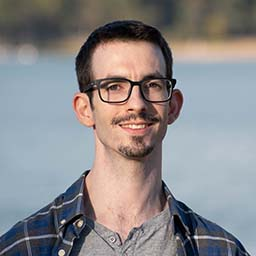
\includegraphics[width=3cm]{victor}
	\end{tabular}
	
	\medskip
	
	%---------------------------------------------------------------------------
	
	\begin{longtable}{p{0.2\textwidth} p{0.8\textwidth}}
		\header{Education}
		2008 -- present & Computer Engineering. \textbf{University of Granada}. \newline
		Final project: \textit{``Remote interpretation of scores on wind 
		instruments''}. \newline
		Supervisor: Prof. Andrés María Roldán Aranda. \\
		2013 -- 2014 & Erasmus scholarship (European Union LLP-Erasmus). \newline
		\textbf{Polytechnic University of Milan}, Italy. \\
		1998 -- 2008 & Elementary Degree to 4\textsuperscript{th} of Professional
		Degree of Piano. \newline
		\textbf{Ángel Barrios Professional Conservatory of music}, Granada. \\
		\\
		\header{Work experience}
		2016 -- present & Security engineer and developer for OSSEC HIDS. \newline
		\textbf{Wazuh Inc.} \\
		2014 -- 2015 & Practices as developer for Android and web apps. \newline
		\textbf{Wap Manía S.L.}\\
		Aug. 2014 & Collaboration in a project to make an isothermal titration 
		calorimeter. \newline
		Department of Physical Chemistry, \textbf{University of Granada}. \newline
		Director: Prof. Antonio Parody Morreale. \\
		2011 -- present & Science, programming and piano support teacher. \\
		\newpage
		\header{Courses and events}
		Jan. 2016 & Workshop about LaTeX and Git. \newline
		\textit{Darwin Eventur}. 50 hours. \\
		2015 -- 2016 & Workshop about SketchUp and Lumion. \newline
		\textit{InterCambia ETSAG}. 20 hours. \\
		Mar. -- May 2015 & Workshop about information resources. \newline
		\textit{University of Granada Library}. 30 hours. \\
		Nov. 2011 & Presentation about open source. \newline
		\textit{Open Source Office}, Granada. 5 hours. \\
		Aug. 2011 & Three-week English course. \newline
		\textit{LTC Eastbourne}, England. 45 hours. \\
		Aug. 2009 & Three-week English course. \newline
		\textit{LTC Eastbourne}, England. 45 hours. \\
		\\
		\header{Personal projects}
		Sept. 2014 & Parallel algorithm for rendering the Mandelbrot set. \\
		Jul. 2014 & Python implementation of a compiler for ARM architecture. \\
		Jul. 2014 & Android Application for image manipulation. \\
		Jan. 2014 & Parallel algorithm for searching prime numbers. \\
		Jun. 2013 & Application for managing a basketball club. \\
		Jan. 2013 & 16 meta-algorithms to resolve the travelling salesman problem. \\
		Feb. 2013 & 4 implementations of the n-queens constraint satisfaction 
		problem in order to compare efficence across programming languages. \\
		Nov. 2012 & Heuristic search algorithm for solving Sudoku-Hex. \\
		Sept. 2012 & Vernam cipher with a Fibonacci LFSR. \\
		Feb. 2012 & Design of a social network for image sharing and 
		manipulation. \\
		Jan. 2012 & 3-D version of the videogame \textit{Arkanoid}. \\
		Nov. 2011 & Graphical interface to design Bèzier curves. \\
		\newpage
		\header{Skills profile}
		Languages & English (advanced) \newline
		Italian (upper intermediate) \newline
		French (elementary) \\
		Programming &
		\begin{subtable}
			C/C++ (expert) \newline
			Java (advanced) \newline
			Python (advanced) &
			C\# (intermediate) \newline
			Prolog (beginner) \newline
			Lisp (beginner)
		\end{subtable} \\
		Frameworks &
		\begin{subtable}
			POSIX \newline
			MPI \newline
			OpenMP &
			Qt \newline
			OpenGL \newline
			Processing
		\end{subtable} \\
		Platforms &
		\begin{subtable}
			Linux \newline
			Windows \newline
			Android &
			Arduino \newline
			Raspberry Pi
		\end{subtable} \\
		Web &
		\begin{subtable}
			PHP \newline
			JavaScript &
			HTML5 \newline
			CSS
		\end{subtable} \\
		Databases &
		\begin{subtable}
			MySQL \newline
			SQLite &
			Oracle
		\end{subtable} \\
		Mathematics &
		\begin{subtable}
			Mathematica &
			MATLAB
		\end{subtable} \\
		Linux & 
		\begin{subtable}
			Shell &
			Git
		\end{subtable} \\
		Text edition &
		\begin{subtable}
			LaTeX &
			Doxygen
		\end{subtable} \\
		Image edition &
		\begin{subtable}
			Adobe Photoshop &
			MAGIX Video Deluxe
		\end{subtable} \\
		3D modelling &
		\begin{subtable}
			SketchUp &
			Lumion
		\end{subtable} \\
		Driving license & Category B (cars) \\
		\\
		\header{Interests and activities}
		2010 -- 2013 & Founding member and pianist in the band \textit{Milestones}. \\
		2010 -- present & Performer as pianist at Musical Evenings. \newline
		High Technical School of Computer Engineering, Granada. \\
		2010 -- present & Blog about computers: 
		\href{http://vikman90.blogspot.com}{vikman90.blogspot.com}. \\
	\end{longtable}
\end{document}

